\section{Magnesium has three stable isotopes with atomic weights of 24, 25, and 26. You are given one mole of enriched magnesium. The block weighs 25.2 grams. You do not know the fractions of Mg-24, Mg-25, and Mg-26 in the block, only the total mass.}

\begin{enumerate}[label=\textbf{\Alph*}.]
    \item Let $p_1$, $p_2$, and $p_3$ be the fractions of Mg-24, Mg-25, and Mg-26 atoms in your sample. Obviously $p_1+p_2+p_3=1$. You also have the constraint that the total mass is 25.2g. Use maximum entropy principles to derive the joint probability distribution $P(p_1,p_2)$ that has the largest entropy given the constraints. (Hint: assume that the measure function $m(x)$ is constant when calculating the entropy of this continuous distribution -- see the formula for the entropy of a continuous probability distribution in Gregory's book. Also, think carefully about the allowed ranges for each variable. The PDF won't depend upon $p_3$ because $p_1+p_2+p_3=1$ determines $p_3$.)

    The formula from Gregory for a continuous distribution with $m$ constant is:

    \begin{align*}
        S_c = -\int P(y) \ln(P(y)) dy + \text{constant}
    \end{align*}

    Or in our case,
    \begin{align*}
        S_c = -\iiint P(p_1, p_2, p_3) \ln(P(p_1, p_2, p_3)) dp_1 dp_2 dp_3 + \text{constant}
    \end{align*}

    And here we have the following constraints:
    \begin{align*}
        p_1+p_2+p_3 &= 1\\
        24p_1 + 25p_2 + 26p_3 &= 25.2 \\
    \end{align*}

    When are both constraints satisfied?
    \begin{align*}
        p_1 + p_2 + p_3 &= 1 \\
        \implies p_3 &= 1 - p_1 - p_2 \\
        24p_1 + 25p_2 + 26(p_3) &= 25.2\\
        \implies 24p_1 + 25p_2 + 26(1 - p_1 - p_2) &= 25.2\\
        24p_1 + 25p_2 - 26p_1 - 26p_2 &= 25.2 - 26\\
        -2p_1 - p_2 &= -0.8\\
        p_2 &= 0.8 - 2p_1\\
        p_3 &= 1 - p_1 - p_2 \\
        \implies p_3 &= 1 - p_1 - (0.8 - 2p_1) \\
        p_3 &= 0.2 + p_1 \\
    \end{align*}

    Use the constraints to get the triple integral down to a single integral:
    \begin{align*}
        S_c &= -\iiint \delta(p_1 + p_2 + p_3 - 1) \delta(p_2 = 0.8 - 2p_1) \\
        &\hspace{2cm}P(p_1, p_2, p_3) \ln(P(p_1, p_2, p_3)) dp_1 dp_2 dp_3 + \text{constant} \\
        &= -\int_0^{p_1} P(p_1') \ln(P(p_1')) dp_1' + \text{constant} \\
    \end{align*}

    Maximize the entropy:
    \begin{align*}
        \frac{dS_c}{dp_1} &= 0 \\
        -\frac{d}{dp_1}\int_0^{p_1} P(p_1') \ln(P(p_1')) dp_1' + 0 &= 0 \\
        \implies P(p_1) \ln(P(p_1)) &= 0 \\
    \end{align*}

    This means either $P = 0$ (not possible here), or $\ln(P) = 0$.
    \begin{align*}
        \ln(P(p_1)) &= 0 \\
        \implies P(p_1) &= 1 \\
    \end{align*}

    To normalize, find the bounds on $p_1$:
    \begin{align*}
        0 &\le p_2 \le 1 \\
        0 &\le 0.8 - 2p_1 \le 1 \\
        -0.8 &\le - 2p_1 \le 0.2 \\
        0.8 &\ge 2p_1 \ge -0.2 \\
        0.4 &\ge p_1 \ge -0.1 \\
        \implies 0.4 &\ge p_1 \ge 0 \\
    \end{align*}

    \begin{align*}
        0 &\le p_3 \le 1 \\
        0 &\le 0.2 + p_1 \le 1 \\
        -0.2 &\le p_1 \le 0.8 \\
        \implies 0 &\le p_1 \le 0.8 \\
    \end{align*}

    Combining those, we see, $p_1 \in [0, 0.4]$. Normalize:
    \begin{align*}
        \int_0^{0.4} P(p_1) dp_1 = 0.4
    \end{align*}

    So our probability distribution is:
    \begin{align*}
        P(p_1) &= 2.5, p_1 \in [0, 0.4]
    \end{align*}

    We could also write this with delta functions if we didn't want to specify a range:
    \begin{align*}
        P(p_1, p_2, p_3) &= 2.5\delta(p_1+p_2+p_3-1)\delta(24p_1 + 25p_2 + 26p_3 - 25.2)\\
    \end{align*}

    \item Suppose we measure $p_1 = \frac{12}{20}, p_2 = \frac{3}{20}, p_3 = \frac{5}{20}$.

    Prior: $P(p_1) = 2.5, p_1 \in [0, 0.4]$

    Likelihood: multinomial with $p_1, p_2 = 0.8 - 2p_1, p_3 = 0.2 + p_1$
    \begin{align*}
        P(n_1, n_2, n_3|p_1, p_2, p_3) &= \frac{n!}{n_1!n_2!n_3!}p_1^{n_1}p_2^{n_2}p_3^{n_3}\\
        P(n_1, n_2, n_3|p_1) &= \frac{n!}{n_1!n_2!n_3!}p_1^{n_1}(0.8 - 2p_1)^{n_2}(0.2 + p_1)^{n_3} \\
    \end{align*}

    Probability of data:
    \begin{align*}
        P(n_1, n_2, n_3) &= \int_0^{0.4} P(p_1)P(n_1, n_2, n_3 | p_1)dp_1 \\
        &= \int_0^{0.4} P(p_1)\frac{n!}{n_1!n_2!n_3!}p_1^{n_1}(0.8 - 2p_1)^{n_2}(0.2 + p_1)^{n_3}dp_1 \\
    \end{align*}

    Posterior (cancel constants):
    \begin{align*}
        P(p_1| n_1, n_2, n_3) &= \frac{P(n_1, n_2, n_3| p_1)P(p_1)}{P(n_1, n_2, n_3)}\\
        &= \frac{P(p_1)\frac{n!}{n_1!n_2!n_3!}p_1^{n_1}(0.8 - 2p_1)^{n_2}(0.2 + p_1)^{n_3}}{\int_0^{0.4} P(p_1)\frac{n!}{n_1!n_2!n_3!}p_1^{n_1}(0.8 - 2p_1)^{n_2}(0.2 + p_1)^{n_3}dp_1}\\
        &= \frac{p_1^{n_1}(0.8 - 2p_1)^{n_2}(0.2 + p_1)^{n_3}}{\int_0^{0.4} p_1^{n_1}(0.8 - 2p_1)^{n_2}(0.2 + p_1)^{n_3}dp_1}\\
    \end{align*}

    \newpage
    If we go any further analytically it might be messy, but here's a plot:

    \begin{center}
        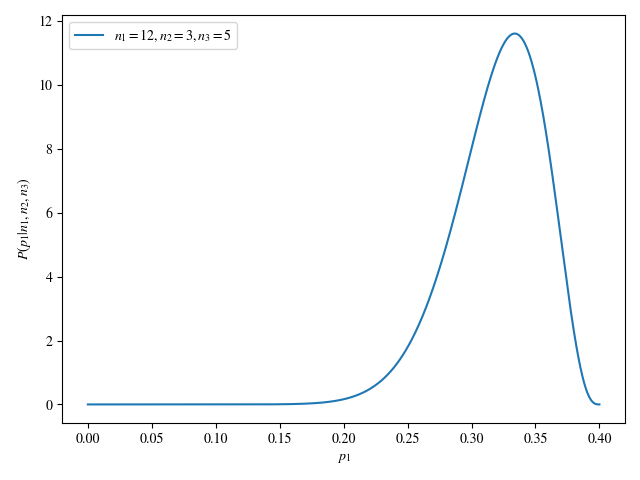
\includegraphics[width=0.9\textwidth]{images/q4_b.png}
    \end{center}

    \newpage
    \item If the data were instead $n_1 = 12, n_2 = 7, n_3 = 1$, what is the posterior? Argue why it makes sense.
    
    It's the posterior from above, with new $n$ values, here's a plot of both:

    \begin{center}
        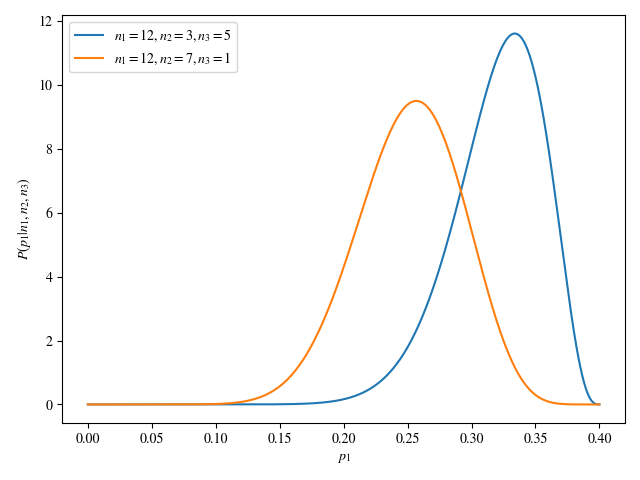
\includegraphics[width=0.9\textwidth]{images/q4_c.png}
    \end{center}

    They're not same, which makes sense since although the posterior doesn't depend on $p_2$ and $p_3$, it does depend on $n_2$ and $n_3$.

\end{enumerate}
